\documentclass[main.tex]{subfiles} % Subfile-Class


% ============================================================================== %
%                            Subfile document                                    %
% ============================================================================== %

\begin{document}

% Template

\subsubsection{Sensorik Strecken Rückverfolgung}

Der Algorithmus setzt vorraus, dass das Gerät immer und zu jeder Zeit seine
Orientierung als absoluten Winkel ab dem Startpunkt weiss und die
zurückgelegten Strecken messen kann. Dieser Abschnitt behandelt, wie der
Pfadfinder eben diese Information sicherstellt.
Abbildung~\ref{fig:Blockschaltbild_StreckenTracken} zeigt schematisch auf, wie
diese Funktion umgesetzt wird. Die danach folgende Beschreibung führt dieses
Schema nochmal aus.

\begin{figure}[h!]
    \centering
    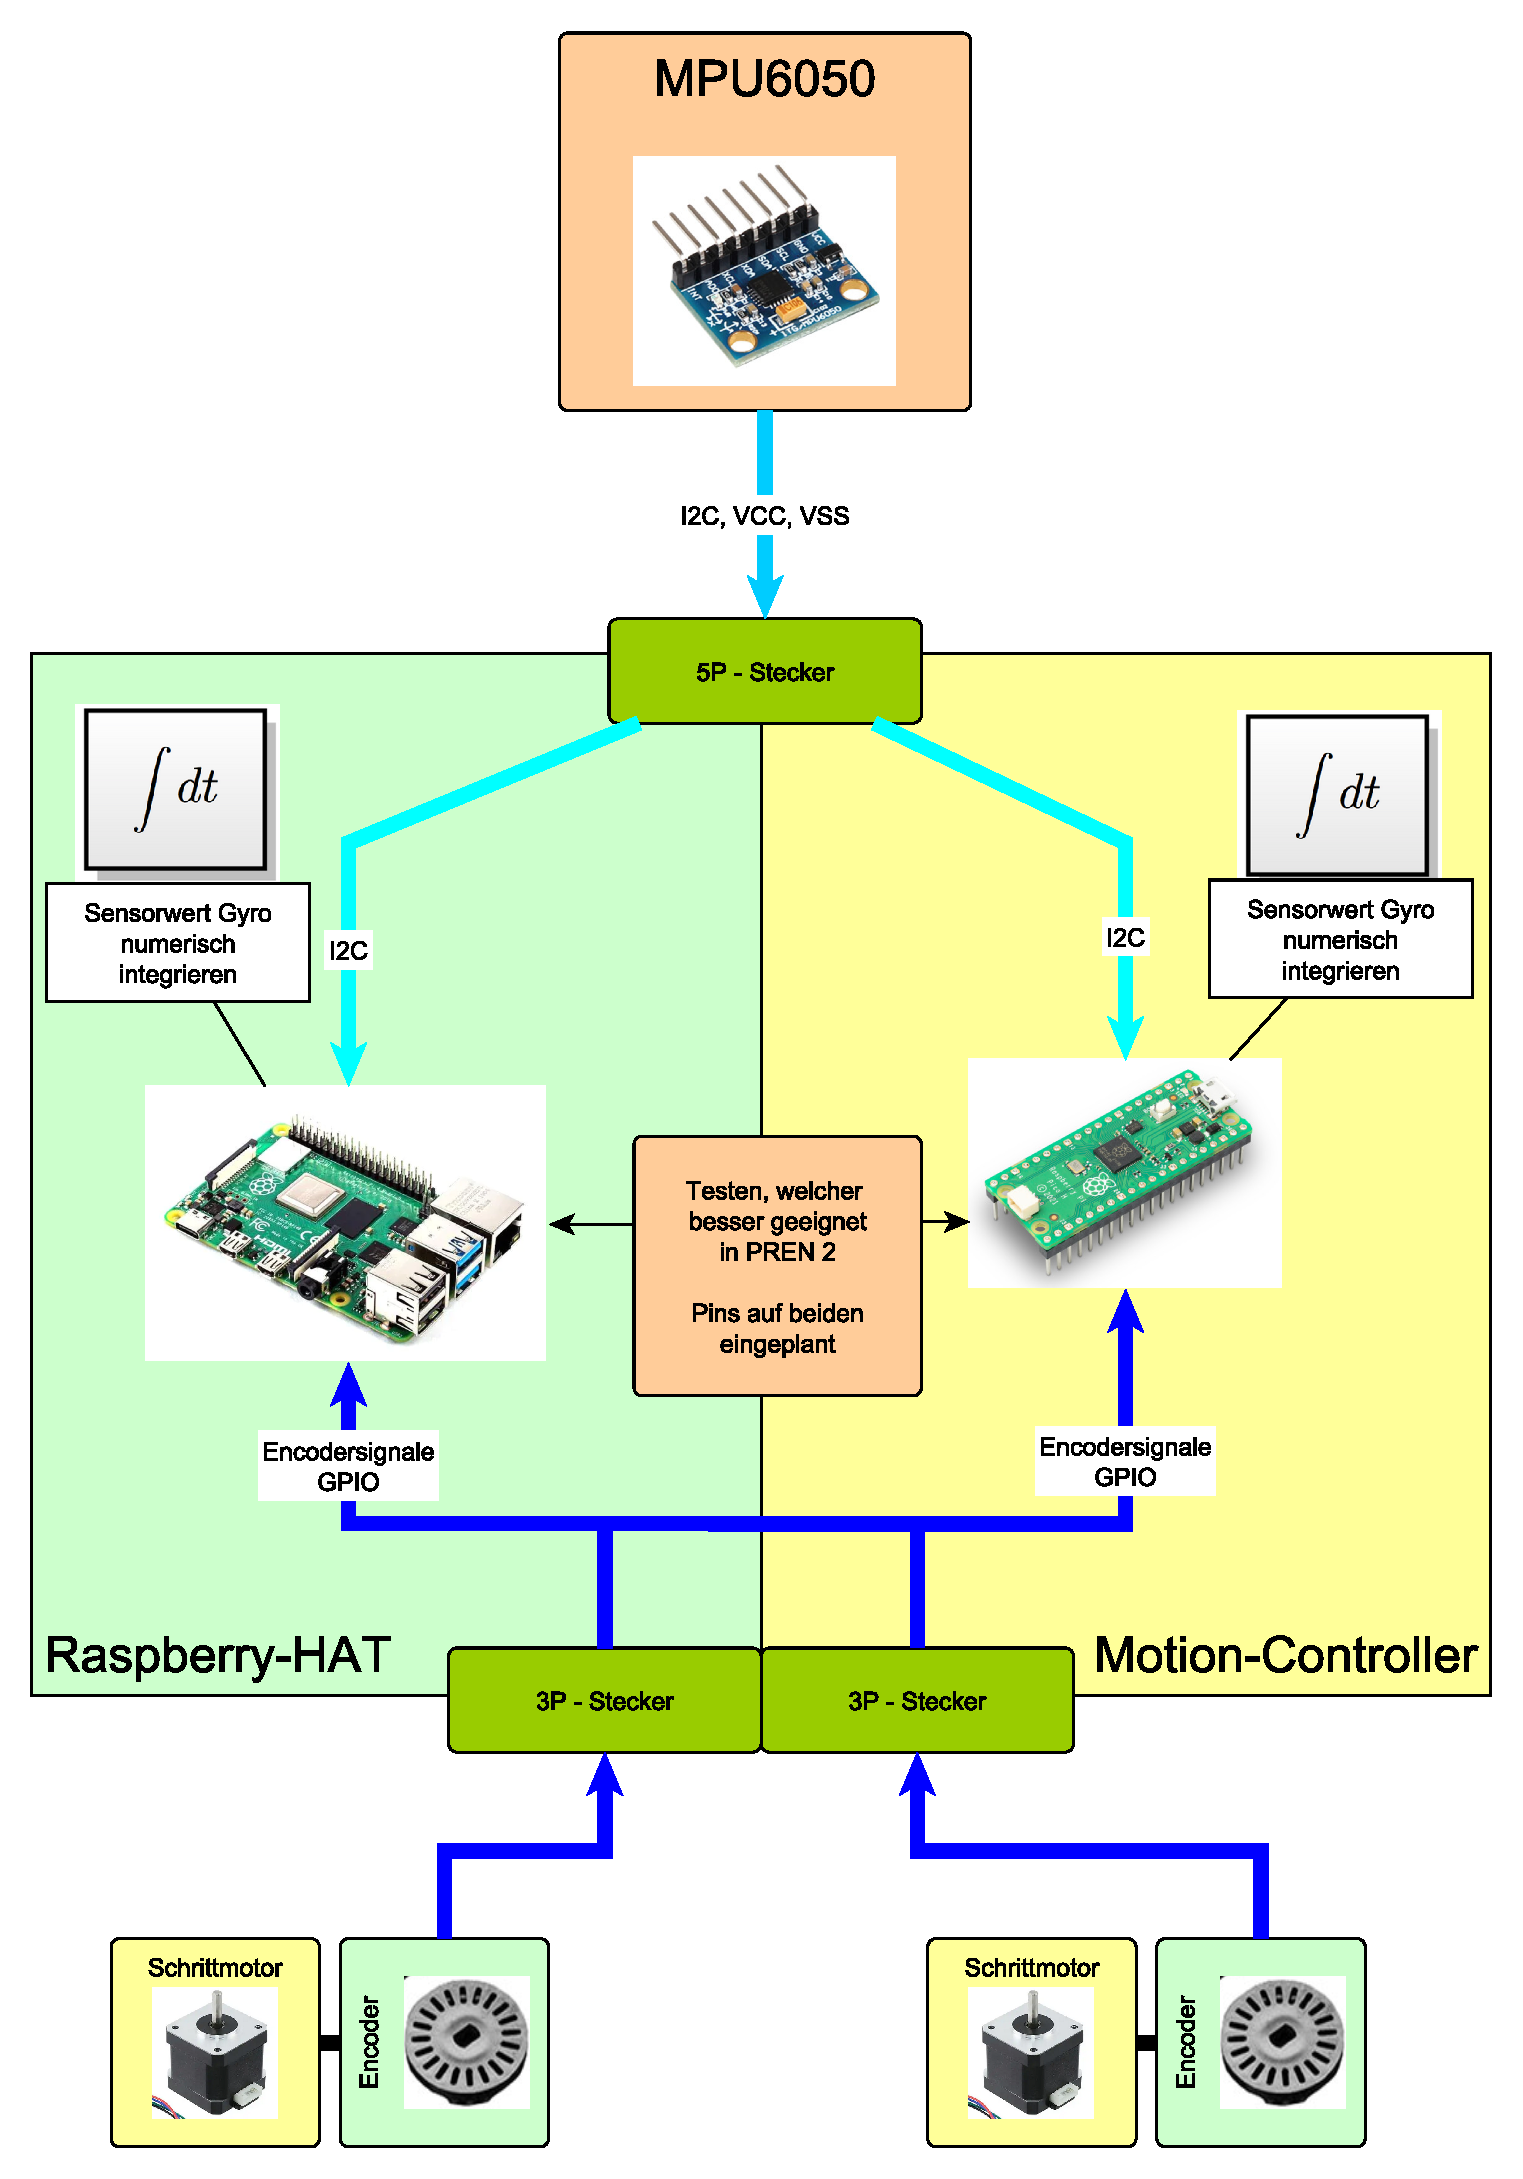
\includegraphics[width=0.75\textwidth]{./fig_Strecke_Tracken/Topologie_MPU6050.pdf}
    \caption{Blockschaltbild Sensorik Streckenrückverfolgung}~\label{fig:Blockschaltbild_StreckenTracken}
\end{figure}

% ===================================================================================
\paragraph{Wineklerfassung}
Der Winkel des Pfadfinders wird, wie in Anhang (REFERENZ!!!!!!!!!!!!!), über
ein Gyroskop ermittelt, welches die Änderungsrate des aktuellen Winkels zu
jeder Zeit erfasst. Eben diese Änderungsrate wird jede $25\mu s$ numerisch
integriert und bringt eine sehr genaue Angabe darüber, in welcher Orientierung
sich das Gerät aktuell befindet.

Mangels Echtzeitfähigkeit ist es nicht sicher, ob der Raspberry Pi in der Lage
ist das Gyroskop ausreichend genau auszulesen. Deshalb wird ein entsprechender
Steckplatz sowohl auf dem Antriebs-Controller, als auch auf dem Raspberry-Hat
vorgesehen, um dies im Nachfolgemodul PREN2 noch zu testen.

\paragraph{Zurückgelegte Strecke}
Wie in der Konzeption (ANHANG !!!!!!!!!) erfwähnt, wird die zurückgelegte
Strecke des Pfadfinders über Encoder ausgezählt. Die Auflösung beträgt (YANNIK
LOCHSCHEIBE???????). In einem zweiten Versuch soll im Folgemodul PREN2 getestet
werden, ob es ausreichen könnte, die zurückgelegten Schritte des
Schrittmotorentreibers für diese Referenz zu verwenden.

\end{document}
